\documentclass[final]{article}
\title{Prognosis of prostate adenocarcinoma metastasis using gene activation profiling}
\author{Christopher C Thompson}
%packages
\usepackage[margin=1in]{geometry}
\usepackage{hyperref}
\usepackage{graphicx}
\usepackage{sidecap}
%path definitions
\graphicspath{{Figures/}}


\begin{document}
\maketitle

\section{Definition}

\subsection{Project Overview}

The prostate is a glandular organ of the male reproductive system that helps to
control urinary and reproductive functions.  According to the charity Prostate
Cancer UK, one in eight British men will  be diagnosed with prostate
adenocarcinoma (prostate cancer, henceforth 'PC') in their  lifetime \cite{PCUK}
Men over 50 years of age are often subjected to routine digital examinations, or
urine test (the Prostate Secreted Antigen, or 'PSA' test) for signs of PC.  However the gold standard
diagnosis is the Gleason test.  In brief, a series of small needle sized
biopsies are taken from the patient's prostate gland.  Each biopsy is processed
and scored by a pathologist for signs of abnormal cell type and
structure.  Gleason scores ranging from 2 to 5 are considered not
malignant, whereas scores ranging from 6-10 are considered malignant and provide
an added estimation of severity \cite{Humphrey04}.

Contrary to some types of cancer, malignancies that remain local within the
prostate are rarely lethal (survival rate of ~99\%).  However, if a malignancy
born of the prostate undergoes distant metastasis (the process of cancer cell
migration to other sites in the body), the survival rate drops to ~28\% \cite{CancerOrg}.
Because of this discrepancy, many men opt for radical prostatectomy (surgical
removal of the entire prostate).  While ensuring prevention of metastasis,
removal of the prostate results in high morbidity, e.g. inability to control
urination, loss of sexual function, etc.

Unfortunately, there are currently no prognostic tests for PC metastasis.  The
patient data  that is typically available at the time of diagnosis is not rich
enough to accurately predict the likelihood of PC metastasis.   A
model that is able to predict whether an untreated malignancy would be likely to
remain locally within the prostate or to metastasize could be an invaluable tool
on whether prostatectomy (and the associated morbidity) is necessary.  To
generate such a model, a more distinguishing set of feature data is required.

One potential solution to this problem is an RNA-seq profile.  In brief, RNA-seq
is a technique that reads and counts RNA sequences in a biological specimen
sample.  What is RNA?   When a gene is activated in a cell, the DNA sequence is
read ('transcribed') into an RNA molecule.  Thus by reading all of the RNA
molecules that exist in a sample, one may determine which genes have been
activated, and to what degree.  A gene count profile is the estimation of
activation for the full set of known human genes.

As metastatic cancer cells behave in drastically different ways than malignant
cells that remain local, there must be an inherent difference in gene activation
between the two cell types.   This difference may be detectable, however there
are likely to be many different genetic paths towards metastasis. Thus it is
unlikely that a single gene could distinguish metastasis state and local
malignancy. The ultimate goal of this project is to determine whether the
RNA-seq profile taken from a cancerous prostate biopsy during initial
presentation and diagnosis, is  sufficient for prognosis of PC
metastasis.

\subsection{Problem Statement}

The primary questions that this project aims to answer are :
\begin{itemize}
\item Can the risk of PC metastasis state be predicted from a gene activation (RNA-seq) profile?
\item so, what genes (individually or in concert) are important for this assessment?
\end{itemize}

The goal of this project is to design a model that predicts the risk of prostate
cancer metastasis using the gene activation profile derived from the patient's
prostate biopsy, taken at the initial Gleason Test diagnosis phase.

To achieve this goal, it is likely that a  significant feature reduction
exercise will be necessary, as each  RNA-seq profile quantifies expression of
20501 human genes.  After feature reduction, a model will be generated to
quantify the risk of PC metastasis (probability from 0 to 1).
Finally, a function or application will be engineered that receives an RNA-seq
profile as an input and outputs a prediction for future metastasis.

\subsection{Metrics}

An appropriate metric for the assessment of class probability prediction is the
Logarithmic Loss (Log Loss) score.

The equation for log loss is : $$ logloss = -\frac{1}{N} \sum_{i=1}^{N} (y_i
*log(p_i) + (1- y_i) * log(1-p_i)) $$ where \textit{p} represents an observations
predicted probability ($0 < \textit{p} < 1$) and \textit{y} represents the actual binomial class
\{0,1\}.

The log loss function provides a penalty score for each predicted observation in
relation to the difference between the actual class {0,1} and predicted
probability (0:1).  Predictions that are both incorrect and confident are
punished harshly.  For instance, were a prediction to call an example as
absolutely true (1) and the example was actually false (0), then infinity would
be returned. Thus, the log loss functions caps predicted probabilities
away from 0 or 1 to  avoid this situation.  An ultra-conservative model that
predicted 0.5 for every observation (effectively not taking either stance in
classification) would have a benchmark log loss score of approximately 0.693147.

\section{Analysis}

\subsection{Data Exploration}

\href{www.http://cancergenome.nih.gov/}{'The Cancer Genome Atlas' (TCGA)} is a
research consortium set up to curate clinical data from thousands of patient
participants, covering an array of cancer types.   Provided data includes basic
clinical information as well as DNA and RNA sequencing of cancer biopsies. These
data sets are updated frequently as new information becomes available.  Thus
each data download represents a snapshot in an evolving data set.

While detailed genomic and RNA sequence data is control-accessed, pre-processed
gene count data is publicly available.  Data can be downloaded via the
consortium  portal or acquired into data frame format using a package in the R
language.  The versions stored in the submission repository are current at
the time of submission.


The clinical data set contains 22 features, of which several are irrelevant
(e.g. all PC patients are 'male').  Of the features, three would be
known at or very near the time of presentation: age, PSA test score, and Gleason
score.  One feature that would also be known but eliminated for ethical reasons is
patient 'race'.  While a higher proportion of Black or Afro-Caribbean men are
diagnosed with PC, the reasons for this are unclear and significant evidence suggests that
race/ethnicity should not be used in cases of genetic / gene activation analysis \cite{Yudel16}.

The primary data set to be used in this project is the gene count matrix.  This
data set provides a value for gene expression level for every known human gene.
The same patient index links the clinical data set to the  gene count data set,
of which 497 are common among the two.

The outcome variable for this project is contained in the clinical data set,
which is 'pathologyNstage'.  This label is composed of 'n0' or 'n1',
representing local versus metastatic cancer, respectively.  The current
percentage of metastatic cases is approximately 16\%.

\begin{SCfigure}
	\centering
	\caption{Frequency of metastasis state ('pathologyNstage') in the TCGA Prostate adenocarcinoma cohort.\label{MetFreq}}
	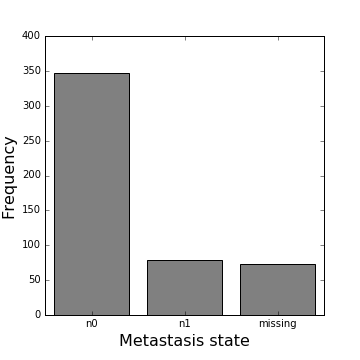
\includegraphics[scale=0.5]{LabelCount}
\end{SCfigure}


The primary data set for this project is the gene count matrix.  This data set
provides a value for gene expression level for every known human gene.  The same
patient index links the clinical data set to the  gene count data set, of which
497 are common among the two.  As the expression values for each patient are not
normalized, an important step prior to analysis was to transform each value to
the transcript count per million reads (TPM).  This transformation normalizes
such that the expression levels for each patient are now comparable.  A test was
run after transformation to ensure that each patient profile totaled 1 million
reads.  The next section will serve to describe the clinical data and provide a
benchmark prognosis rate using information available to a doctor at
presentation.

When grouped by Gleason score, it is also evident that metastasis rates increase
as the severity of cancer increases (Figure 2).  This is  intuitive, yet clearly
not sufficient to determine whether a specific cancer, regardless of Gleason
score, will metastasize or not.  To illustrate, cancers that have been rated at
a Gleason score of '9' are still more likely to belong to the 'n0' class than
the metastasis class.

\begin{SCfigure}
  \centering
  \caption{Frequency of metastasis state grouped by Gleason score.\label{fig:preGSHist}}
  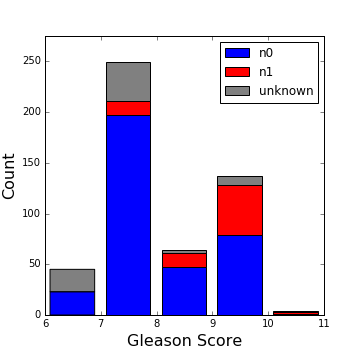
\includegraphics[scale=0.5]{GleasonHist}
  %\caption{Frequency of metastasis state grouped by Gleason score.\label{fig:preGSHist}}
\end{SCfigure}

\subsection{Exploratory Visualization}

An overview analysis shown in Figure \ref{fig:FDist} of the gene count dataset revealed that
some genes appear to be differentially activated in the two metastasis states.
This indicates that there are genes that could be used for predictive purposes
and validates the project rationale.

\begin{figure}[h]
  \centering
  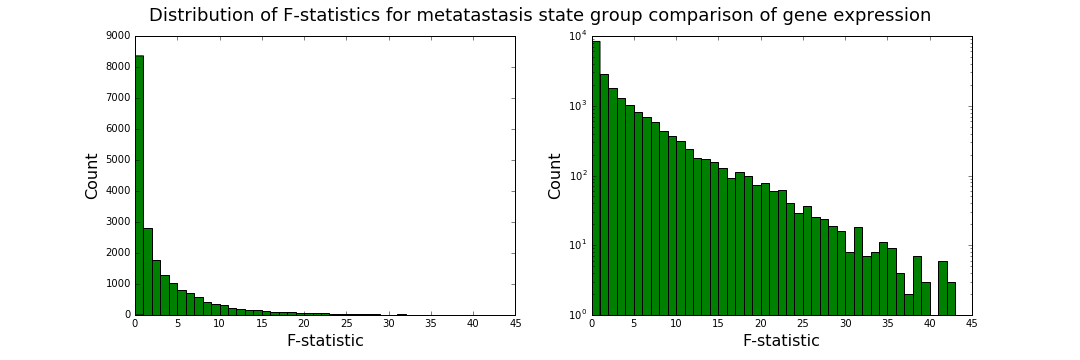
\includegraphics[width = \textwidth]{FDist}
  \caption{Distribution of F-test statistics for the comparison of gene expression levels between the 'n0' and 'n1' metastasis states.\label{fig:FDist}}
\end{figure}

\subsection{Algorithms and Techniques}

The basic outline for project completion is as follows:
\begin{enumerate}
\item Feature selection (filter mechanism)
\item Feature compression into a lower dimensional set
\item Train the probabilistic-classification algorithm
\item Measure performance of the trained algorithm on an independent validation ('test') set
\item Compare model performance to the benchmark model performance
\end{enumerate}

The feature reduction exercise will utilize Random Forest Classifier, not as a
classification algorithm, but as a method to measure the ability of each gene to
separate the dataset by metastasis class.  Given noisy data, decision trees (and
thus Random Forest) classifiers are prone to overfitting, so parameter limits on
the tree depth and the minimum number of samples that can be split will be defined.
The top portion of genes will be subset into a new reduced data set and carried
into the next project phase.

The reduced feature data set will be compressed further using Principle Component
Analysis (PCA).  PCA is an unsupervised learning technique that transforms a
dataset into its principle components - \textit{i.e.} the orthogonal vectors within the
data that explain the greatest amount of its variance.  By selecting the
the most important components, several features may be combined into a lower
number without significant loss of information.  How many principle components
will be carried into the algorithm training will depend on the amount of variance
each component can explain.  For example, if the first principle component that
explains 95\% of the dataset variance, it would not be necessary to bring any other
principle components forward for further analysis.

The probabilistic-classification algorithm chosen for this task is the logistic
regression ('logit') model.  This algorithm was chosen for its inherent ability
to assess the probability of a binary outcome (\textit{i.e.} metastasis or local
malignancy) based on continuous input variables.

Important parameters for the Logistic Regression are:

* regularization equation ('penalty') - 'l2'
* solver - 'liblinear'
* regularization term ('C') - '1'

Of the options for the regularization equation parameter, the 'l2' algorithm was
preferable to the 'l1' as the input set contained a relatively small set of
features  (just 3).  For training situations with a large number of variables,
the 'l1' equation is more suitable, as it generates sparsity (\textit{i.e.} limits the
number of features that  significantly contribute the the logistic function
outcome).  The solver 'liblinear' is most appropriate with small datasets, such
as this one.  The regularization term  was initialized at 1, but would be
optimized later using cross-validation.


\subsection{Benchmark}

As personalized medicine (\textit{e.g.} use of a patient's specific genetic or gene
activation information for therapeutic decisions) has not been established in
mainstream therapy, a benchmark for use of RNA-seq data for prognosis of
metastasis was not available.  Hypothetically, the most conservative model which
predicts every test sample as having 50% chance of metastasis would yield a log
loss score of ~0.69314.

To establish a more fair benchmark for comparison, a logistic regression model
(see methodology below) that incorporated the clinical information that would
normally be known at the time of diagnosis was generated.  These features were
'age', 'PSA score', and 'Gleason score'.

\begin{figure}[h]
  \centering
  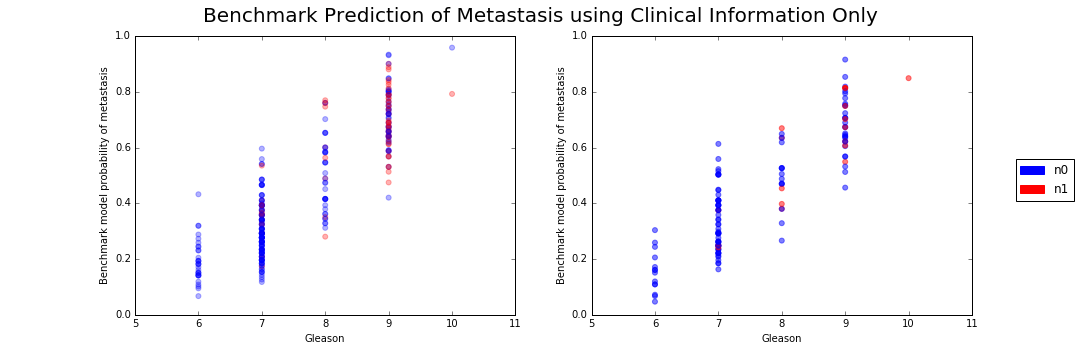
\includegraphics[width=\textwidth]{benchmark}
  \caption{Visualization of a benchmark logistic regression predictive model performance.\label{fig:benchScat}}
\end{figure}

The coefficients for the three features in the model training exhibited that
Gleason score was by far the most predictive (0.855), and that age and
interestingly PSA score (which is the current default test that doctors rely on
for PC risk)  provided very little use in classification.  Figure 5
(left) shows the relationship between Gleason score and the benchmark model's
prediction of metastasis.  Figure 5 (right) shows the distribution of metastasis
probabilities, grouped by actual metastasis state.

The log loss score from this benchmark analysis ranged from 0.571 - 0.644 across 5 different runs (\ref{tab:performance}), and
thus was marginally more useful than a '50\% model'.

\section{Methodology}

\subsection{Source Files}

The datasets were retrieved from the TCGA portal using an R package,
\href{https://cran.r-project.org/web/packages/TCGA2STAT/index.html}{TCGA2STAT},
and written in \href{https://github.com/wesm/feather}{feather} format to be
uploaded into the python environment.  The R script and feather files are
available in this project's GitHub repository
\href{https://github.com/CCThompson82/MLE\_capstone}{MLE\_capstone}.  All
algorithms were imported from the
\href{http://scikit-learn.org/stable/}{scikit-learn} library, version 0.17.

\subsection{Data Preprocessing}

Samples with a Gleason score of 6 were homogenous in metastasis state (all
'n0'). Therefore, any sample of Gleason score equal to 6 where the metastasis
label was missing, 'n0' was imputed for the missing label.  This assumption is grounded
in the  procedures followed by urologist upon Gleason screening - those with low
grade  malignancy are usually not screened from metastasis and this is probably
the  source of missing data labels in the TCGA cohort.  This step allowed more
efficient use of a rather small dataset.  Given a much bigger data set, then
this assumption would not be necessary, and  all cases with missing label could
be excluded.  Indeed, for cases scored 7-10 on the Gleason scale where no labels
were included in the clinical data were excluded from further analysis.

\begin{SCfigure}
  \centering
  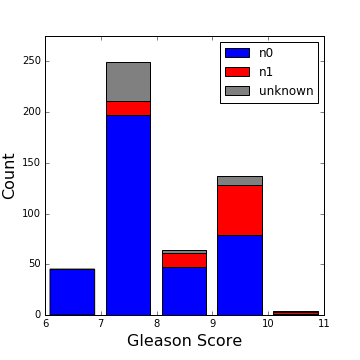
\includegraphics[scale=0.5]{GleasonHist2}
  \caption{Distribution of known clinical features grouped by metastasis state (blue: 'n0', red: 'n1').\label{fig:postGSHist}}
\end{SCfigure}

The gene count data retrieved from the TCGA portal was in an intermediary
format.  While the raw RNA-sequence reads had been processed into gene
activation estimations, each specimens profile required normalization for
cross-comparison.   Therefore, the initial gene count dataset was transformed to
transcripts per million (TPM) format.  This dataframe ('X') was the base upon
which further feature reduction and test train splitting would be performed.

\subsection{Implementation}

Feature reduction was completed in two steps.  The first was to utilize the
generation of a \href{http://scikit-learn.org/stable/modules/generated/sklearn.ensemble.RandomForestClassifier.html#sklearn.ensemble.RandomForestClassifier}{Random Forest Classifier} to supply information regarding the
importance of each gene in the separation of metastasis states.  As the Random
Forest model was not intended for actual classification purposes (due to the
small sample size of the dataset), only key default parameters were altered.
Specifically, the maximum tree depth was limited to 3 nodes, and the minimum
number of samples that could be split was limited to 30.  These parameter choices
were instrumental in preventing any form of extraordinary variance.  The 'Gini
Importance' of each feature was retrieved from the model and the genes ranked
in the order of importance.

Originally, the top \textit{k} number of genes were retained for the
input dataset, however the set of genes was not 100\% stable.  Some genes, such as
\textit{gne} were present in every case, each run resulted in a slightly different selection
of genes.  To address this selection instability, the Gini Importance selection
process was iterated across 5 different random seeds, and the genes present in the top
\textit{k} in every iteration were kept.  In this solution, k was set to 100 and resulted
in a relatively stable selection of ~16-22 genes that would regularly enter the
next phase of the project.

This k-gene set was scaled to standard mean and unit variance using the sklearn
\href{http://scikit-learn.org/stable/modules/generated/sklearn.preprocessing.StandardScaler.html#sklearn.preprocessing.StandardScaler}{Standard Scaler}.

The second phase of Feature reduction was \href{http://scikit-learn.org/stable/modules/generated/sklearn.decomposition.PCA.html#sklearn.decomposition.PCA}{Principle Component Analysis}
compression. A further compression was performed in which PCA was utilized to
transform the k-feature dataset into its principle components.  The contribution
from the k subset of genes in each of the first three principle components is visualized
in Figure 6.

\begin{figure}[h]
  \centering
  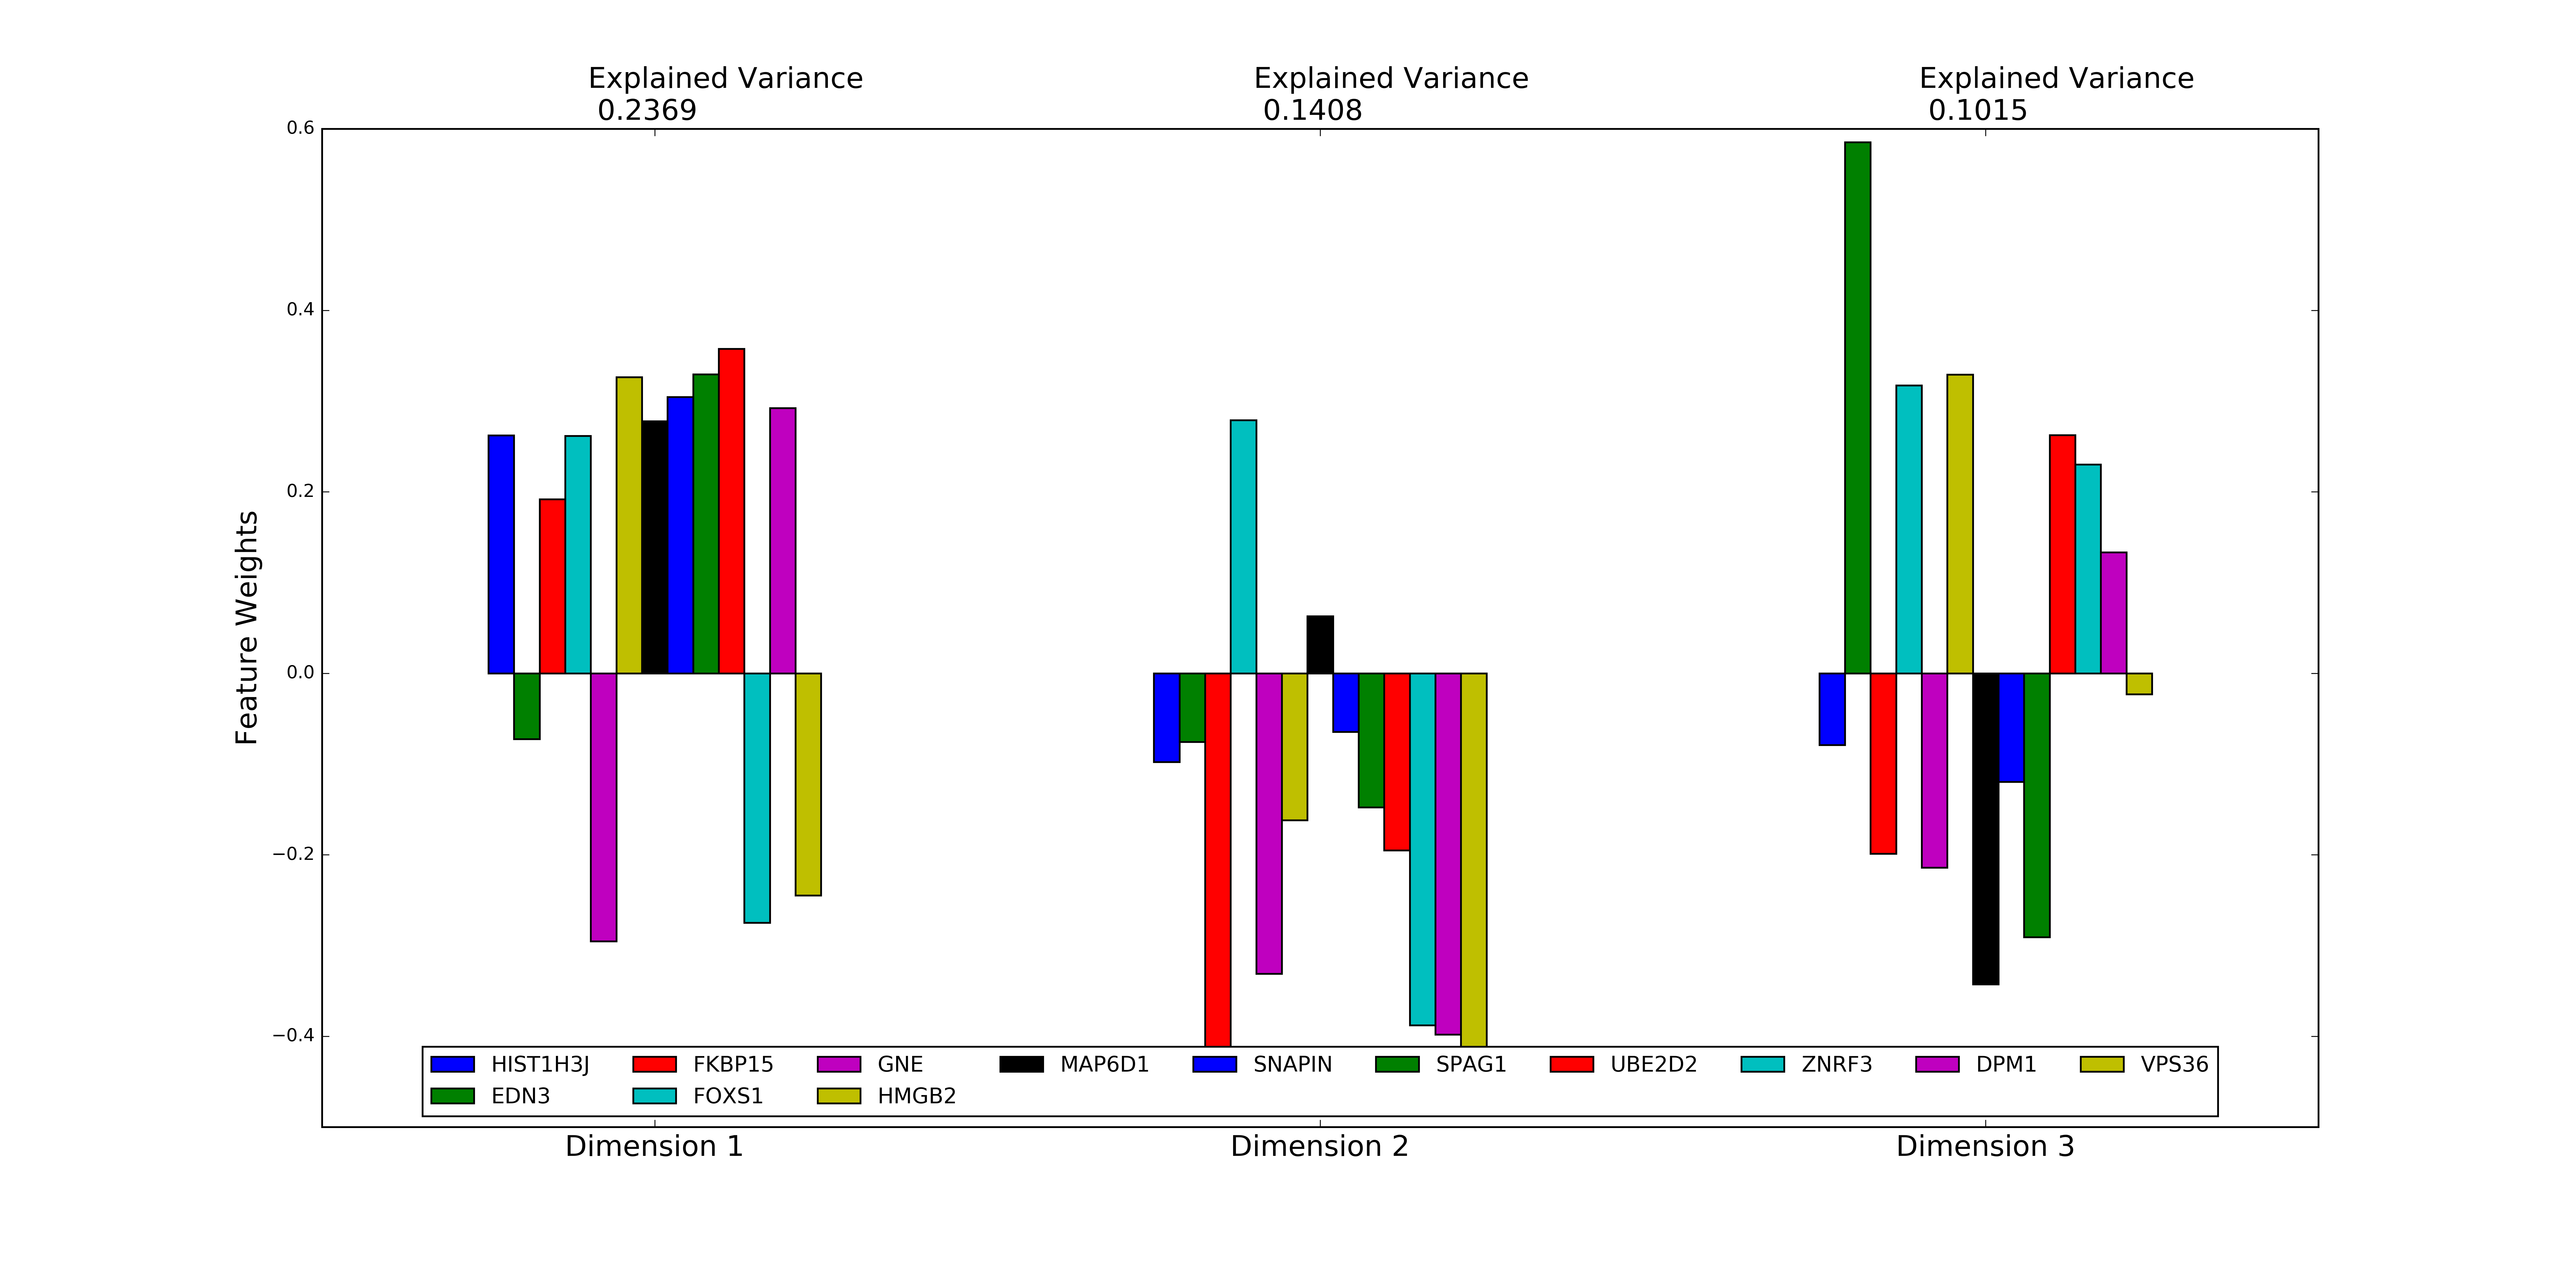
\includegraphics[width=\textwidth]{pcaEV}
  \caption{Explained variance and Gene feature contribution to the first three principle components of the PCA transformation.\label{fig:pcaEV}}
\end{figure}

This 3-feature dataset was then partitioned using the same indices from the
first \href{http://scikit-learn.org/stable/modules/generated/sklearn.cross_validation.train_test_split.html}{Train Test Split}
that was performed prior to the benchmark model generation.  In detail, this
split  partitioned 70\% of the samples into the training set, with 30\% being held
out for validation.  The  data was stratified by Gleason score, which was used
as a surrogate measure for cancer severity. While not a perfect solution, this
decision was made to ensure that 'easy' (\textit{e.g.} mild or extremely severe
malignancies) and 'difficult' (\textit{e.g.} malignancies on the border between
moderate and severe) cases would be distributed equally.  Another option would
have been to stratify by  metastasis label (see 'Reflection' section for  %set up reference label pair here
discussion on this decision).

The training data set was then fed into a
\href{http://scikit-learn.org/stable/modules/generated/sklearn.linear_model.LogisticRegression.html}{Logistic
Regression} For this learning, the class-weight parameter was set to 'balanced'
in order to guard against confounding effects of the unbalanced label set in
model performance.  The regularization ('C') parameter was left at the default
value of 1.  The C term is inversely proportional to the penalties awarded for
misclassified samples. As this dataset appears to be noisy from graphical
analysis, I hypothesized a higher regularization term may increase performance
of the model for future optimizations.  The solver for the algorithm was kept at
the default 'liblinear' function which is most useful against smaller datasets,
such as the one in this project.

Results were visualized using graphs generated with the \href{http://matplotlib.org/index.html}{matplotlib}
package.  Performance of the
logistic regression model was tested against the held-out test set using the
\href{http://scikit-learn.org/stable/modules/generated/sklearn.metrics.log_loss.html#sklearn.metrics.log_loss}{log loss}
metric.  For references, the \href{http://scikit-learn.org/stable/modules/generated/sklearn.metrics.fbeta_score.html}{F$\beta$ score ($\beta$ := 2)}
and \href{http://scikit-learn.org/stable/modules/generated/sklearn.metrics.matthews_corrcoef.html}{Matthews Correlation
Coefficient}
scores are also listed, though they describe the performance of the algorithm to
correctly classify metastasis state.  Both the graphical analysis and metric
reports were generated for each testing cycle using the scripts supplied in the
\href{https://github.com/CCThompson82/MLE_capstone/tree/master/Support%20Files}{'Support Files'}
folder in the GitHub repository.

\subsection{Refinement}

In order to optimize the C parameter, or to determine whether the default was
indeed optimal,  a \href{http://scikit-learn.org/stable/modules/generated/sklearn.linear_model.LogisticRegressionCV.html#sklearn.linear_model.LogisticRegressionCV}{Logistic Regression CV}
classifier generated using 4 fold cross-validation across a 10-log range for C.
Performance was measured using \href{http://scikit-learn.org/stable/modules/generated/sklearn.metrics.log_loss.html#sklearn.metrics.log_loss}{log loss}
as the  scoring function.

The next step in model optimization was to feed back the Gleason score, shown to
be the most important explanatory variable in the benchmark analysis.  It was
unclear whether adding another feature would contribute to variance or improve
generalization.

\section{Results}

\subsection{Model Evaluation and Validation}

\subsubsection{Final Model}

The final logistic regression model receives 2 feature variables:

\begin{enumerate}
\item Gleason score
\item the first 3 PCs from a k-gene subset of expression values
\end{enumerate}

The coefficients for these features were routinely equivalent, indicating they
contribute roughly evenly to dependent variable prediction.  The optimal
regularization parameter was regularly determined as the maximum value tested,
which is an indication of noisy (\textit{i.e.} not linearly separable) data.

\begin{figure}[h]
  \centering
  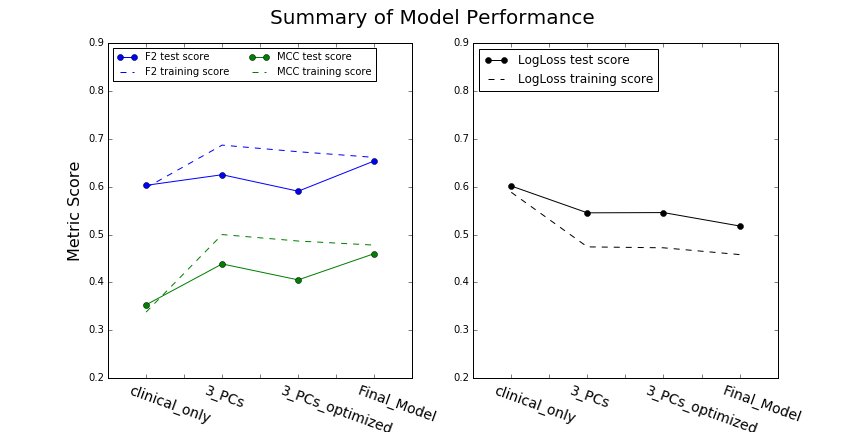
\includegraphics[width=\textwidth]{FF}
  \caption{Summary of the change in metric score over the optimization course of the project.  The final model, that incorporates a single principle component with Gleason score performs better than the benchmark model in three metrics tested.\label{fig:FM}}
\end{figure}

The error / accuracy rate of three performance metrics was often similar
between the training sample and test sample set predictions, indicating the
model was not over-fit.  As only 2 feature  variables were incorporated into the
training of the final model, the possibility of bias was present.  However

\subsubsection{Test set Validation}

\begin{table}[h]
\centering
\caption{Performance across 5 random seeds\label{tab:performance}}
\begin{tabular}[h]{ r c c c }
\hline
Seed & Final Model LogLoss & Benchmark LogLoss & Improvement over Benchmark (\%) \\  \hline
1 & 0.496309 & 0.605505 & 18.0 \\
12 & 0.479994 & 0.618392 & 22.4 \\
123 & 0.556008 & 0.621997 & 10.6 \\
1234 & 0.51460 & 0.615772 & 16.4 \\
12345 & 0.467942 & 0.595507 & 21.4 \\
\hline
\end{tabular}
\end{table}

This project's strategy was to leave out 30\% of the original dataset to use as a
true validation of the models' generalization capability.  The final model test
set log loss score ranged from 0.467 to 0.508 across five different random state
seeds, indicating that modification of the training and test set samples did not
affect outcome of model performance.

\subsection{Justification}

The final logistic regression model was always more accurate in predicting the
probability of PC  metastasis than the benchmark model.  Over the
five consecutive runs described above, an average improvement of 20.8% in log
loss score was achieved over the starting benchmark score.

\begin{SCfigure}
  \centering
  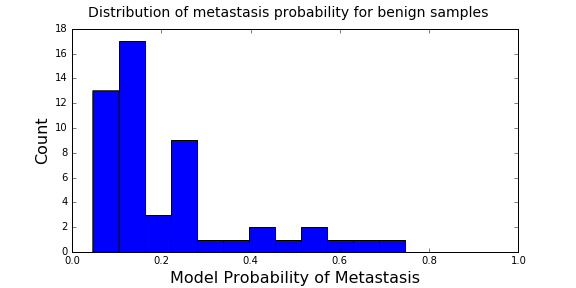
\includegraphics[scale = 0.5]{Sensitivity}
  \caption{\label{fig:Sensitivity}Analysis of risk from matched, benign controls from the TCGA cohort data reveal that the final model is stringent.  Samples from this cohort were taken from benign areas of patient prostates where malignancies were present.  The majority of samples are predicted with a low probability of metastasis.}
\end{SCfigure}

As analysis of sensitivity, a metastasis risk function was implemented and tested
against unlabelled samples, the presumed 'non-metastatic' samples, and matched
benign controls from the TCGA cohort study.

\section{Conclusion}

\subsection{Free-Form Visualization}

A function was written that accepts an RNA-seq gene count profile (in TPM
format), and outputs the model risk for metastasis.  This function was applied
to every sample for which no label was given and showed that a significant
portion of patients in the cohort exhibit a high level of risk for metastasis.

\begin{figure}[h]
  \centering
  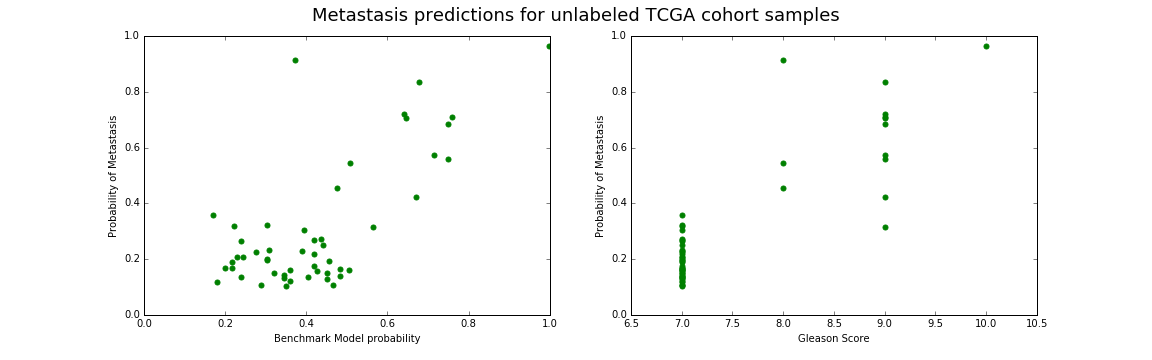
\includegraphics[width=\textwidth]{missing}
  \caption{\label{fig:missing}Metastasis predictions for unlabeled TCGA cohort samples.  TCGA cohort patient samples that did not include a metastasis label and were Gleason range 7-10 were omitted from model learning and validation.  Samples are subjected to the risk analysis function and plotted against the benchmark model prediction (left) and Gleason score (right).}
\end{figure}

\subsection{Reflection}

\subsubsection{Objective}

The purpose of this project was to generate a model capable of supplying a
patient and doctor with a metric for risk of PC metastasis that was
more useful than simple use of the 'Gleason Score'.  To accomplish this, RNA-seq
(gene activation profile) was explored as a potential inroad into personalized
therapy for newly diagnosed PC patients.  There were several issues
that made this task difficult:

\begin{enumerate}
\item Small, wide sample data - the effective
dataset (containing Gene Activation profile and a metastasis label) was 446
samples by 20501 gene features.
\item 'Inaccurate' / 'Pre-mature' data labelling -
The TCGA cohort is regularly updated and those listed as non-metastatic at the
time of update could become metastatic at a later date.
\item Noise in the data -
no single gene or biomarker had been reported as capable of efficiently
separating non-metastatic and metastatic cancers(corroborated in this project,
Figure \ref{fig:separate}).
\end{enumerate}

Thus from a machine learning perspective, it was clear from the project's onset
that feature reduction and appropriate model selection would be paramount to
success.

\subsubsection{Feature Selection}

There are many techniques for feature reduction.  One avenue explored was
feature elimination via a wrapping mechanism.  However this approach was very
slow and provided inconsistent results in which features and how many features,
were important. A different approach was to utilize the
training of an ensemble Random Forest classifier, not for its use in
classification, but in order to access its assessment of which genes were most
informative in separation of the metastasis classes.  An iterative process was
utilized to stabilize the gene set upon which PCA transformation would be performed. Implementation of this feature was not essential for increased final model
validation performance, thought it did reduce the run to run variation in predictive
performance.

Importantly, visualized individually, none of this reduced k-gene set could separate the metastasis
state linearly.

\begin{figure}[h]
  \centering
  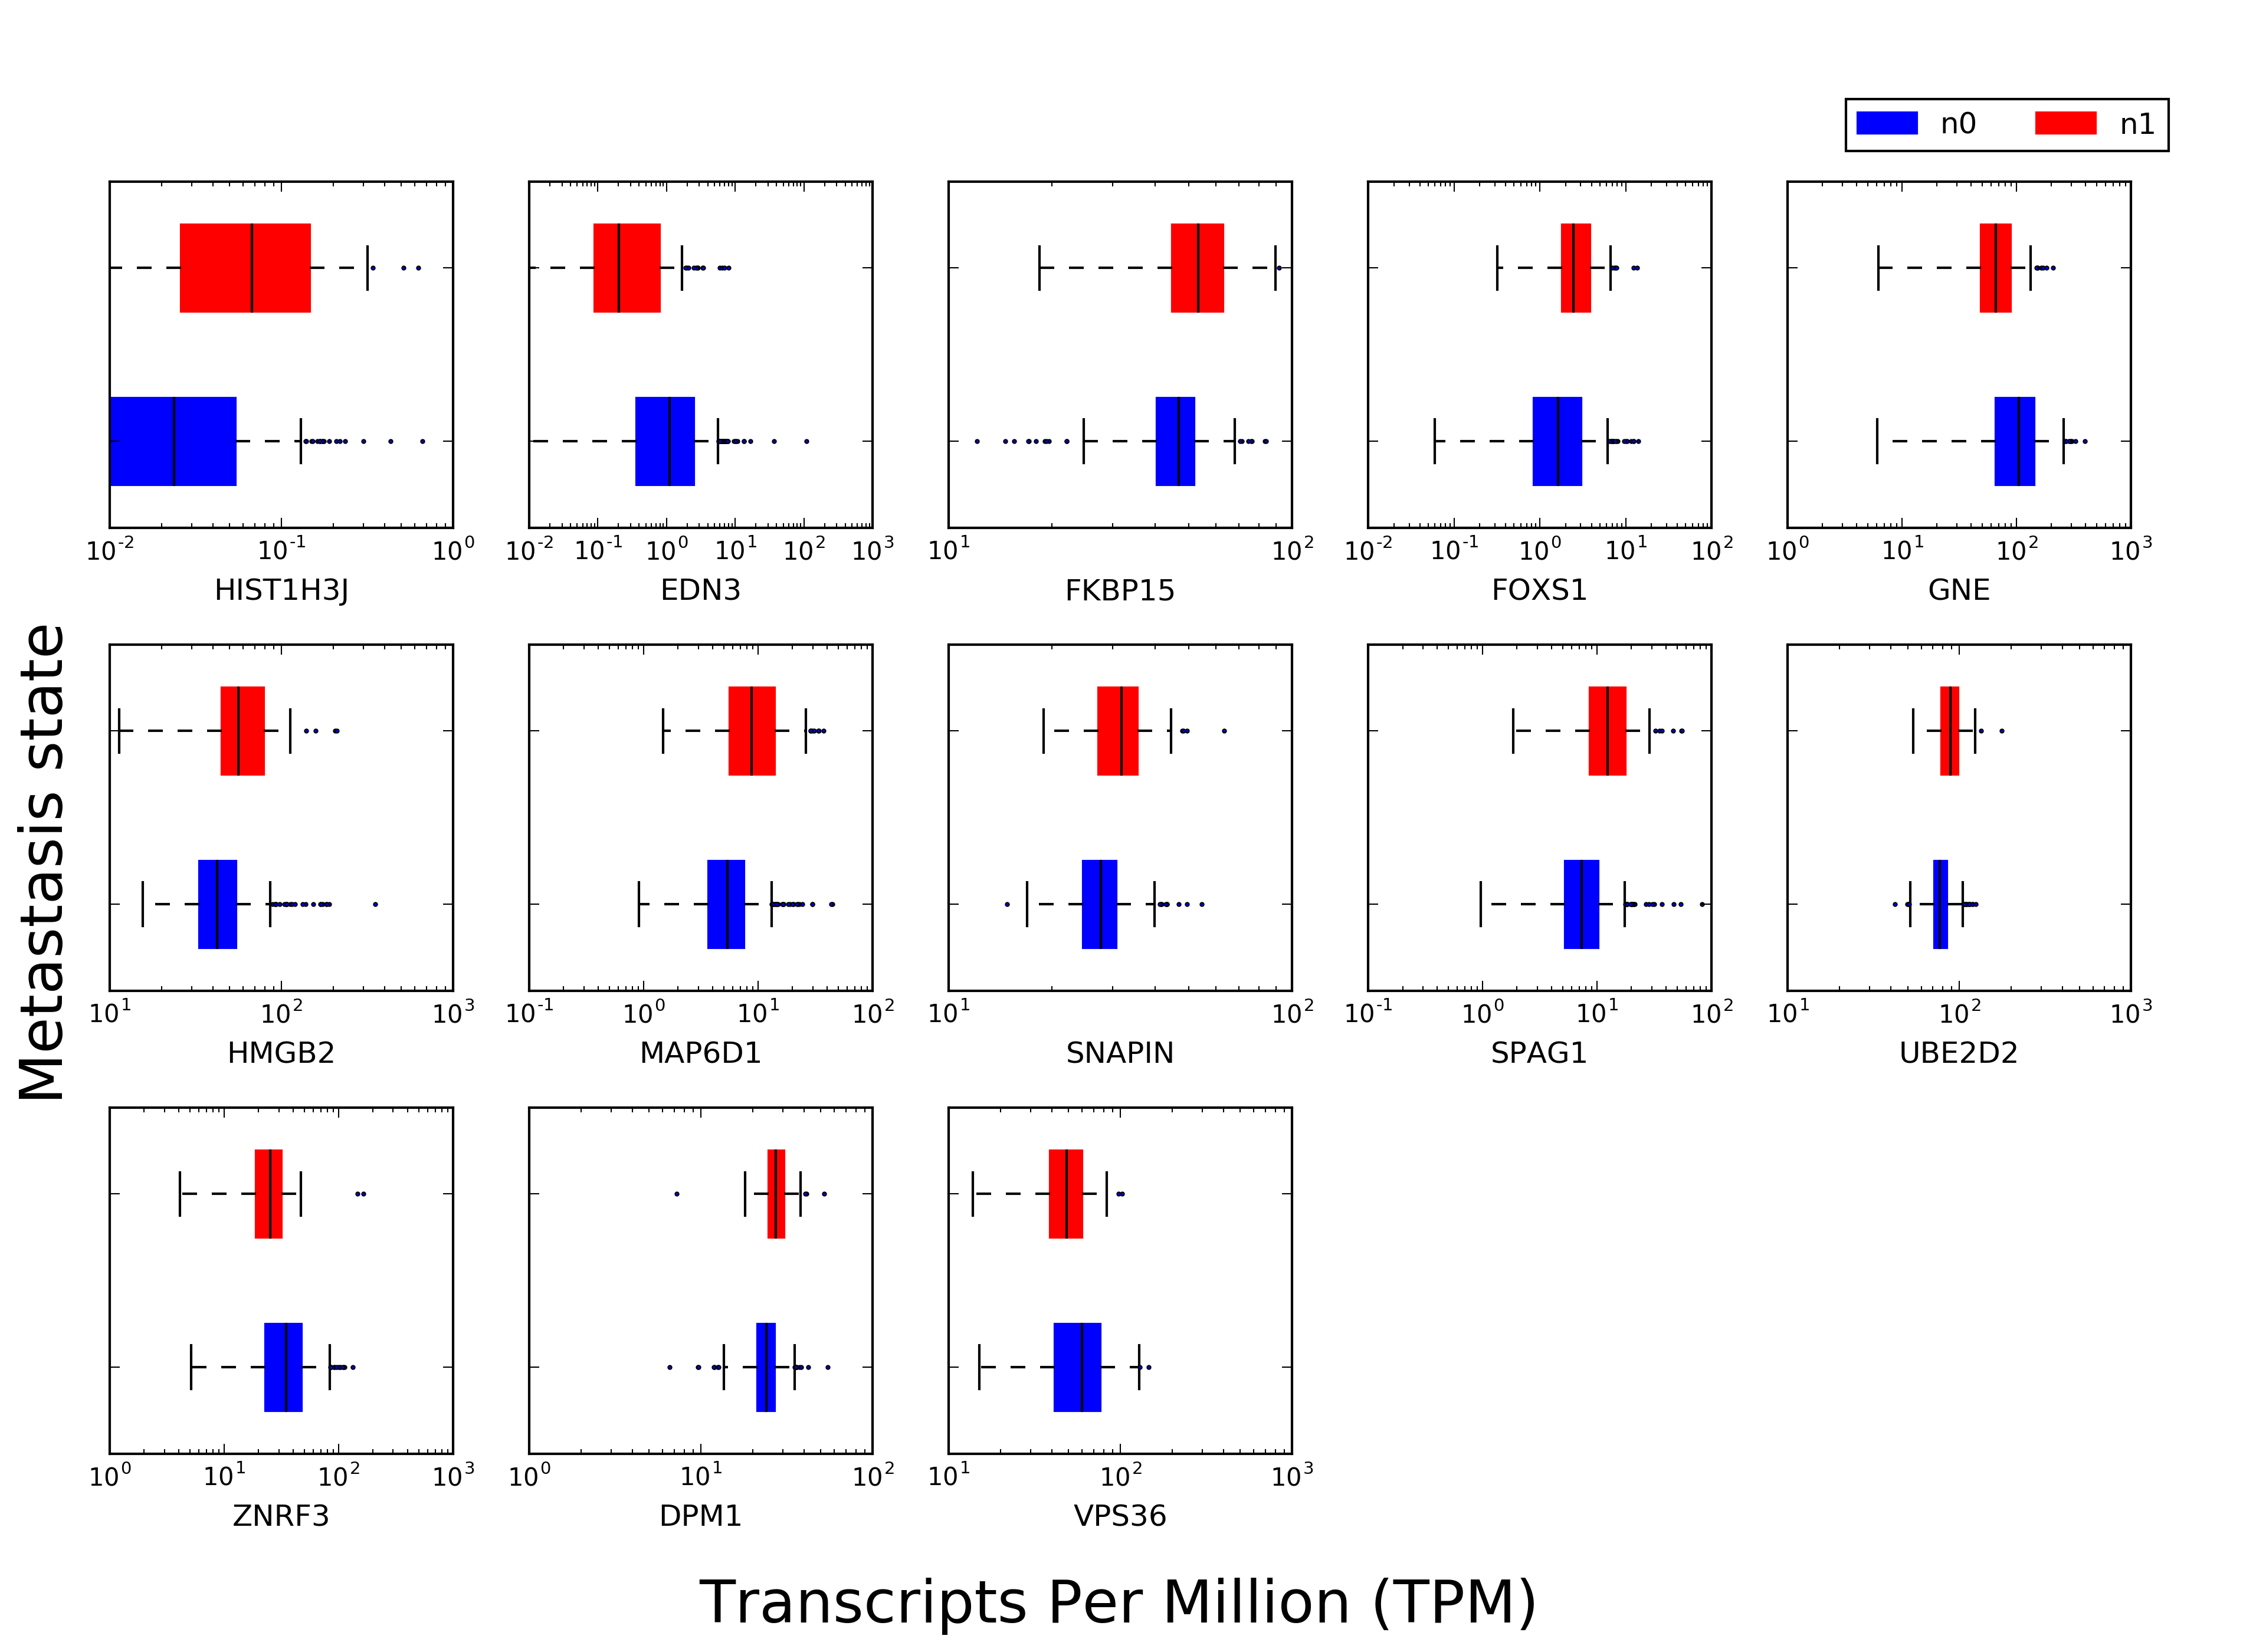
\includegraphics[width=\textwidth]{boxplots}
  \caption{\label{fig:separate}Genes with the highest 'Gini Importance' scores were still not able to distinguish metastasis class.}
\end{figure}

The initial plan at this point was to provide the full complement of principle components to the logistic regression classifier as training data, and
subsequently use each component's coefficient to  assess which were most able to
explain the independent variable in a \href{http://scikit-learn.org/0.15/modules/generated/sklearn.feature_selection.RFECV.html#sklearn.feature_selection.RFECV}{Recursive Feature Elimination}
wrapping function.  However, graphical analysis of the principle component scatter matrix, grouped by
metastasis state (Figure \ref{fig:pcaScatter} ) curiously showed that the first principle
component seemed to generate distinct gaussian distributions for each of the metastasis states, despite the fact that PCA is an unsupervised technique.  This result was consistent independent of
whether 5 through 500 genes were 'Gini' selected for PCA transformation.

How could this be?  This result would be expected if a transformation technique
such as linear discriminant analysis (LDA) had been employed, as LDA uses data
label in order to determine the component vectors where class label is
discriminated the most.  PCA, on the other hand, is an unsupervised technique
and had generated what appeared to be a discriminant component in the absence of
label information.  However, upon reflection, it is perhaps not surprising that
the eigenvector where the most variance in the data subset was contained (\textit{i.e.}
the first principle component) would separate the class labels, given that
\textit{only genes where a 'significant' difference in gene expression between the
class labels} were retained and provided to the PCA model.

By creating a pipeline from the  Gini Importance filter directly into the PCA
transformation, something similar to
\href{http://scikit-learn.org/0.16/modules/generated/sklearn.lda.LDA.html}{Linear
Discriminant Analysis} had been generated.  Indeed, exploration of an supervised
LDA compression of the 20-feature set yielded a similar level of performance in
the final model compared to compression via Gini Importance to PCA pipeline.

\begin{SCfigure}
  \centering
  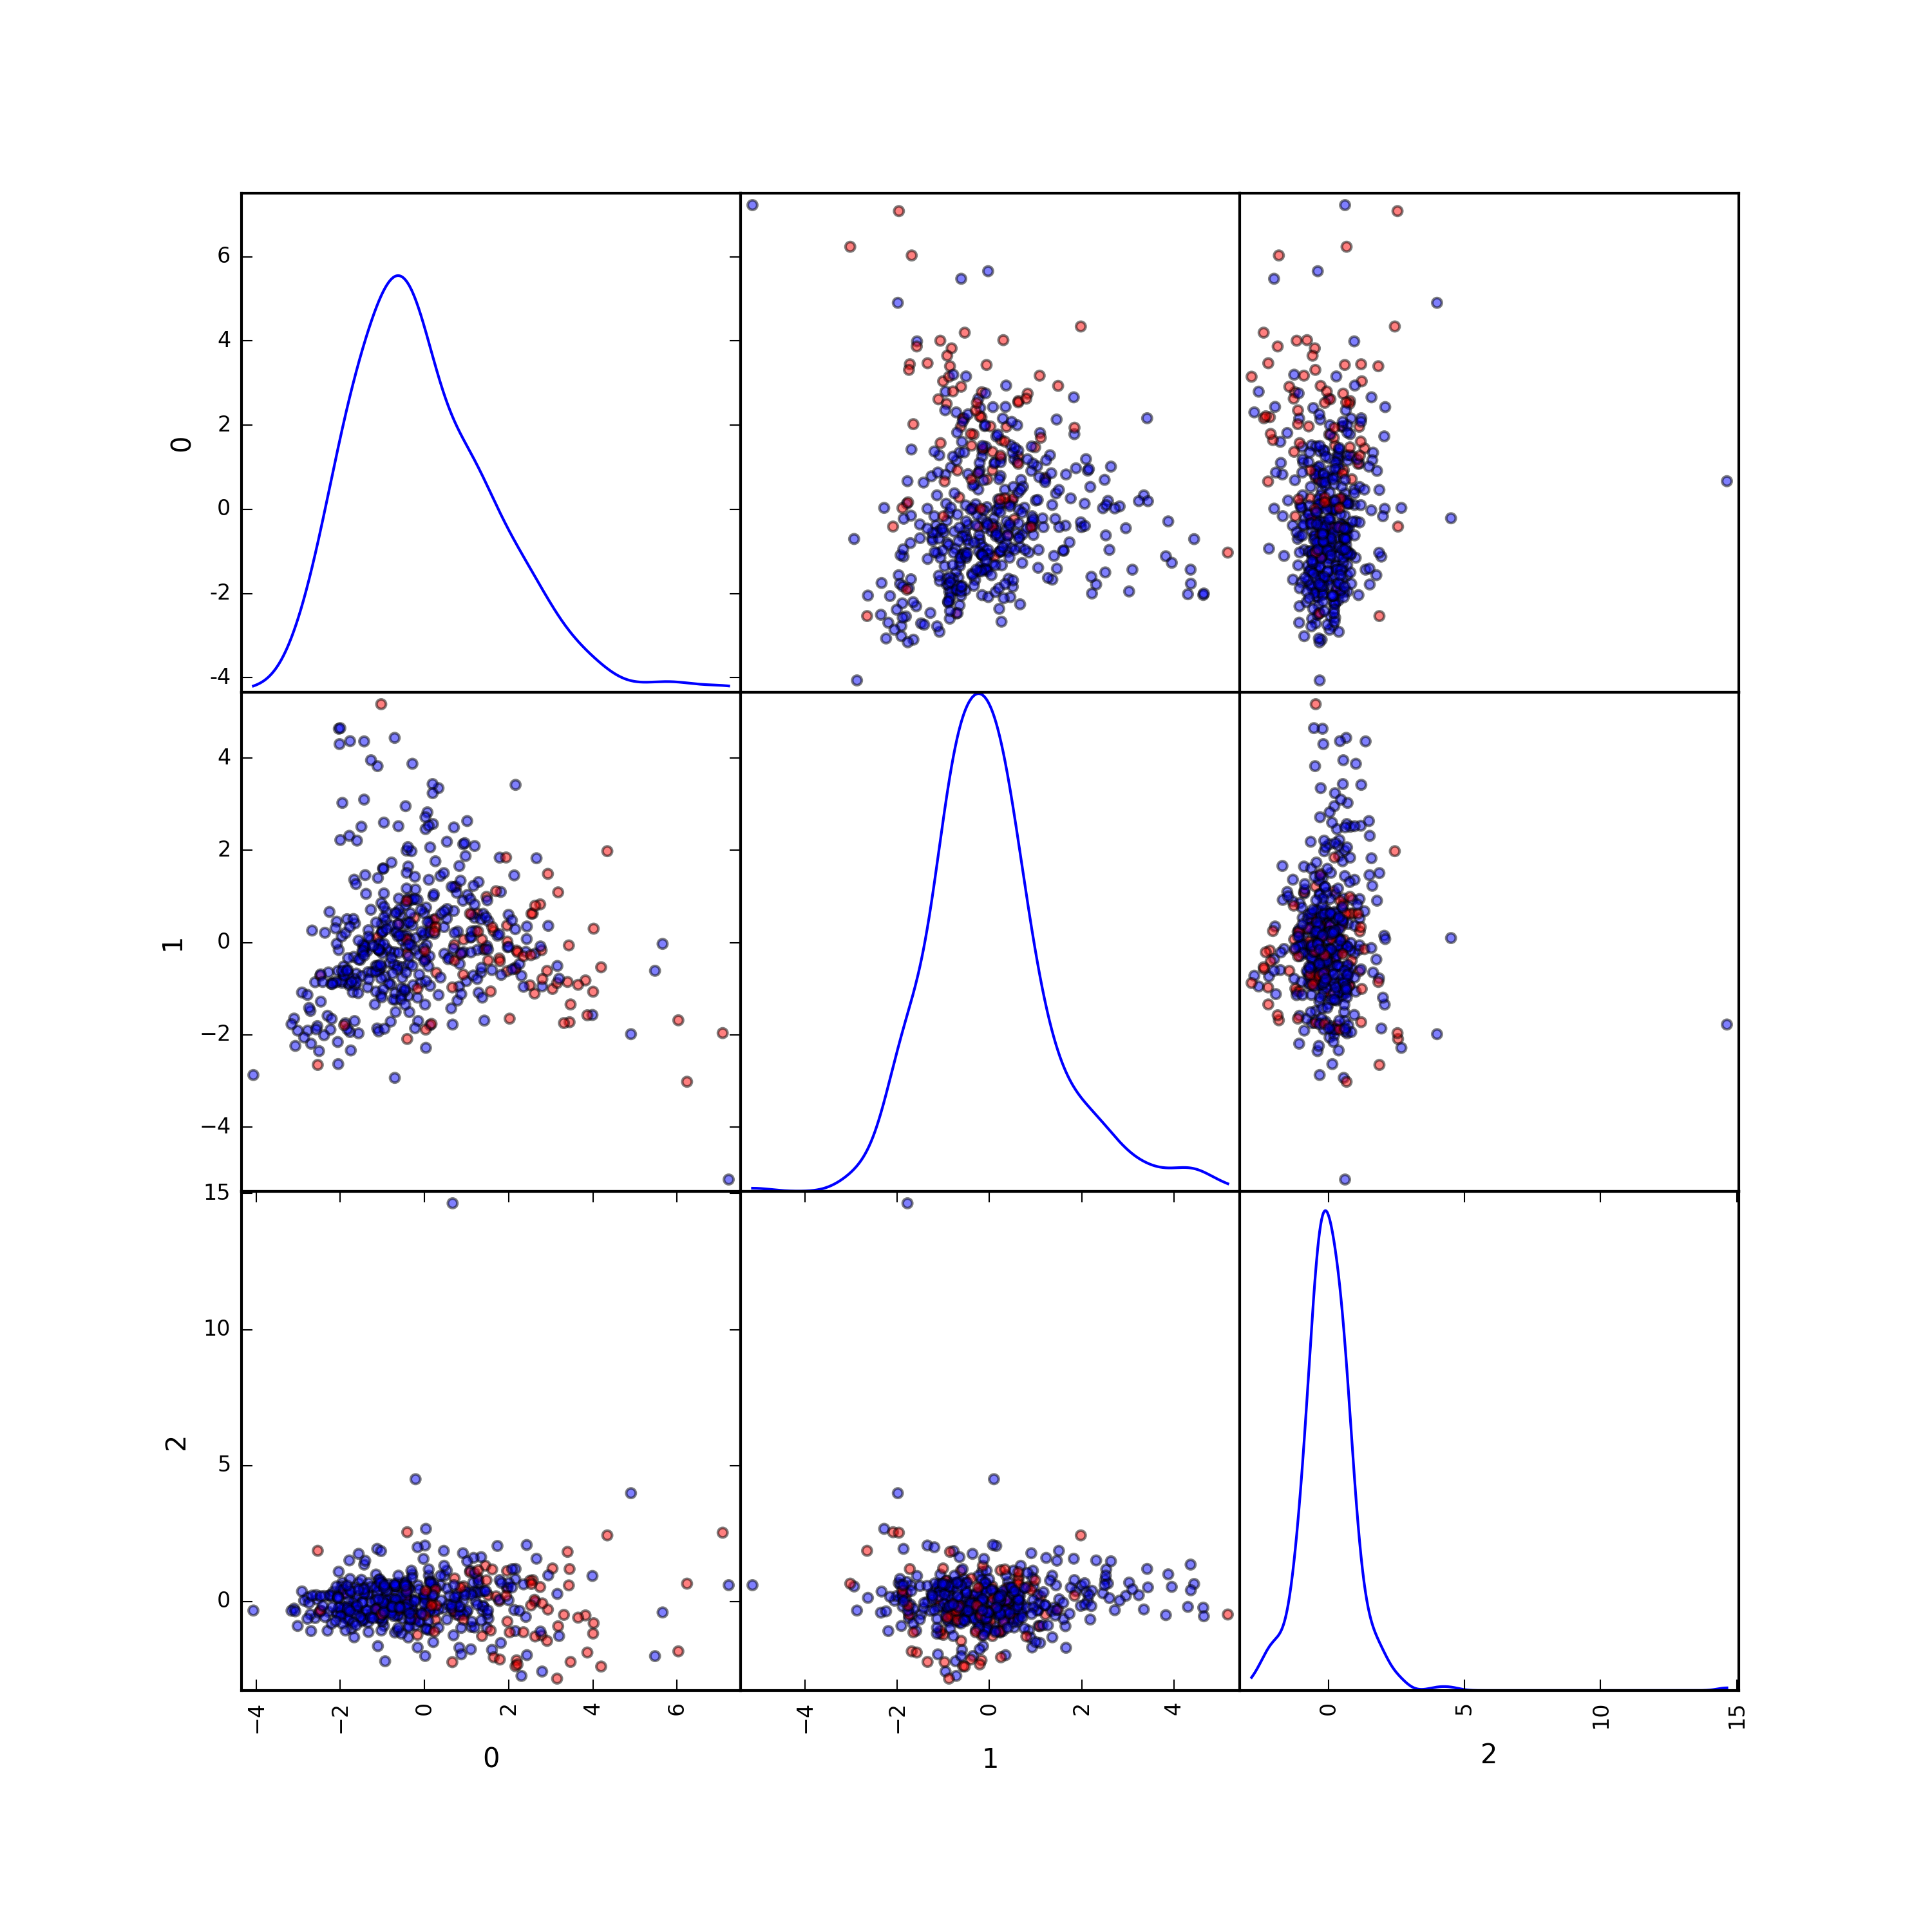
\includegraphics[scale = 0.5]{pcaScatter}
  \caption{\label{fig:pcaScatter}Analysis of PCA transformation of a k-gene feature subset.  The first principle component of PCA transformation separates metastasis state more efficiently than any single gene from the input set.  The second and third principle components are also shown for reference.}
\end{SCfigure}

The 3-component feature set taken from this transformation was split on the same indices that were generated in
the training and validation sets used in the benchmark analysis.  This was done
to aid in model to model comparisons within each run.  To note, this split was
originally stratified on the y-label (metastasis state).  However, after
observing moderately inconsistent results for final model validation
performance, the decision was made to stratify by Gleason score (Cancer
severity) of the samples.   This decision ensured that difficult cases - those
in the middle range of severity - were equivalently distributed among the
training and test sets, vastly reducing the run to run variation.

\subsubsection{Model Selection}

Having completed a feature selection and compression technique, in which at
least the first principle component seemed capable of distinguishing among
metastasis class via graphical analysis (**Figure 11**), a logistic regression
classifier was chosen as the predictive model.  Logistic regression was
preferred  to other hyperplane-based techniques, such as support vector
machines (SVM) due to the noise that was expected in the compressed dataset.
SVM classifiers attempt to define the hyperplane by which the margin between
the class labels is maximized.  In situations where data is not easily
separable, this result can be unstable, and  at times, arbitrary.  Moreover,
SVM does not provide a true probability of class assignment, as was the
objective of the project.  In contrast, logistic regression assumes that no
feature  is capable of explaining the outcome variable, but that the
combination of features  should be able to provide a probability of class
assignment.  This assumption holds true for the RNA-seq dataset employed in
this project.  Moreover, as the objective of this project was to provide a
probability of metastasis, the output of logistic regression classifier is
perfectly suited.

\subsubsection{Training and Optimization}

Separate Train and Test indices were stratified based on cancer severity prior
to the benchmark analysis and the final PCA compressed (3-components) were
subset into these indices.  Logistic regression classifier was trained and
optimized on the Train set, prior to validation on the Test set.  Gleason score
was added as a feature to this model and the 2nd and 3rd principle components
were eliminated from the model after determining that they did not contribute to
model performance.

The final release version of the code was run across 5 seeds and performance in
the primary metric (log loss), and secondary metrics (F2 and MCC) were recorded,
compared to the benchmark.

\subsubsection{Model Performance}

In every run tested, the performance of the final model exceeded performance of
the benchmark model by at least 14\% in log loss score.  The pipeline exhibited
in this project could be re-appropriated for other types of RNA-seq based
classifications.  By looking for individual genes whose activation level explain
a certain condition, researchers may be missing the opportunity to provide
valuable disease prognosis.  Instead, by performing a feature selection and
compression, researchers may be able to predict disease more regularly at the
sacrifice of knowing \textit{exactly} what genes are causal.

Importantly, I hypothesize that as the TCGA cohort study is updated
longitudinally, its performance will be more accurate.  This is due to the
nature  of analyzing an on-going cohort trial.  In the context of a machine
learning problem,  sample labels will only move in one direction (from
'non-metastatic' to 'metastatic', never \textit{vis-a-versa}).  Therefore those patient
samples predicted with a high  probability of metastasis, currently labeled as
non-metastatic, would be correctly classified in future validation.

Unfortunately in the context of the TCGA cohort study, the link between patient
and barcode has been broken for ethical reasons, meaning that such patients with
high risk  can not be identified for extra care in monitoring metastasis.


\subsection{Improvement}

There is still bias in this model due to the small sample size.  Increased
number of specimens could allow more resolution / stability in feature selection
and  compression.  For each iteration of the code, a handful of genes selected
from the 'Random Forest filter' is altered, though 10-15 remain identical.

Evidence here and elsewhere suggests that no gene or principle component could
be capable of separating  metastasis state classes, and thus logistic regression
is an excellent long term  model for prediction.  However, it is possible that
other sources of information  could help improve model accuracy, including
genetic or epigenetic specimen data.  Ultimately only increasing the sample size
will be able to significantly increase the resolution for PC cancer metastasis
prediction.

\section{References}

\begin{thebibliography}{1}
  \bibitem{PCUK}
    Prostate Cancer UK,
    http://prostatecanceruk.org/prostate-information,
    Accessed 01-August-2016.
  \bibitem{Humphrey04}
    Humphrey PA.
    (2004)
    \emph{Gleason grading and prognostic factors in carcinoma of the prostate},
    \textbf{Mod Pathol}.
    17,
    pp 292-306.
  \bibitem{CancerOrg}
    Cancer.org,
    http://www.cancer.org/cancer/prostatecancer/detailedguide/prostate-cancer-survival-rates,
    accessed 01-August-2016.
  \bibitem{Yudel16}
    Yudell M, Roberts D, Desalle R, \& Tishkoff S.
    (2016)
    \emph{Taking race out of human genetics},
    \textbf{Science}
    351,
    pp 564-565.
\end{thebibliography}
\end{document}
